
Die Methode der Diffusion, ist zu beobachten wie sich ein Stoff im Schnee ausbreitet. Für den Vorversuch wurde der Schnee unter ein Stereo Mirkoskop plaziert. Der Versuch dauert etliche Minuten. Um zu verhindern, dass der Schnee von der warmen Raumluft aufgeschmoltzten wird, ist der Schnee in einer Röhre aus Eis platziert. Während das -10 grädige Eis langsam schmiltz, kann der Versuch durchgeführt werden. Die Auswertung bei dem Vorversuch ist optisch, es wird beobachtet wie sich blaue Tinte im Schnee ausbreitet. Eine Kombination dieses Ansatzes mit der Leitfähigkeitsmessung ist möglich, wenn ein leiteder Stoff eingesetzt wird.

Auch dieser Ansatz wird stark von der Geometrie des Schnees beeinflusst. Wieviel flüssiges Wasser vorhanden ist, ist sekundär zu wie die Eiskristalle miteinander verbunden sind. Deswegen wird dieser Ansatz nicht weiter verfolgt.

\begin{figure}
    \centering
    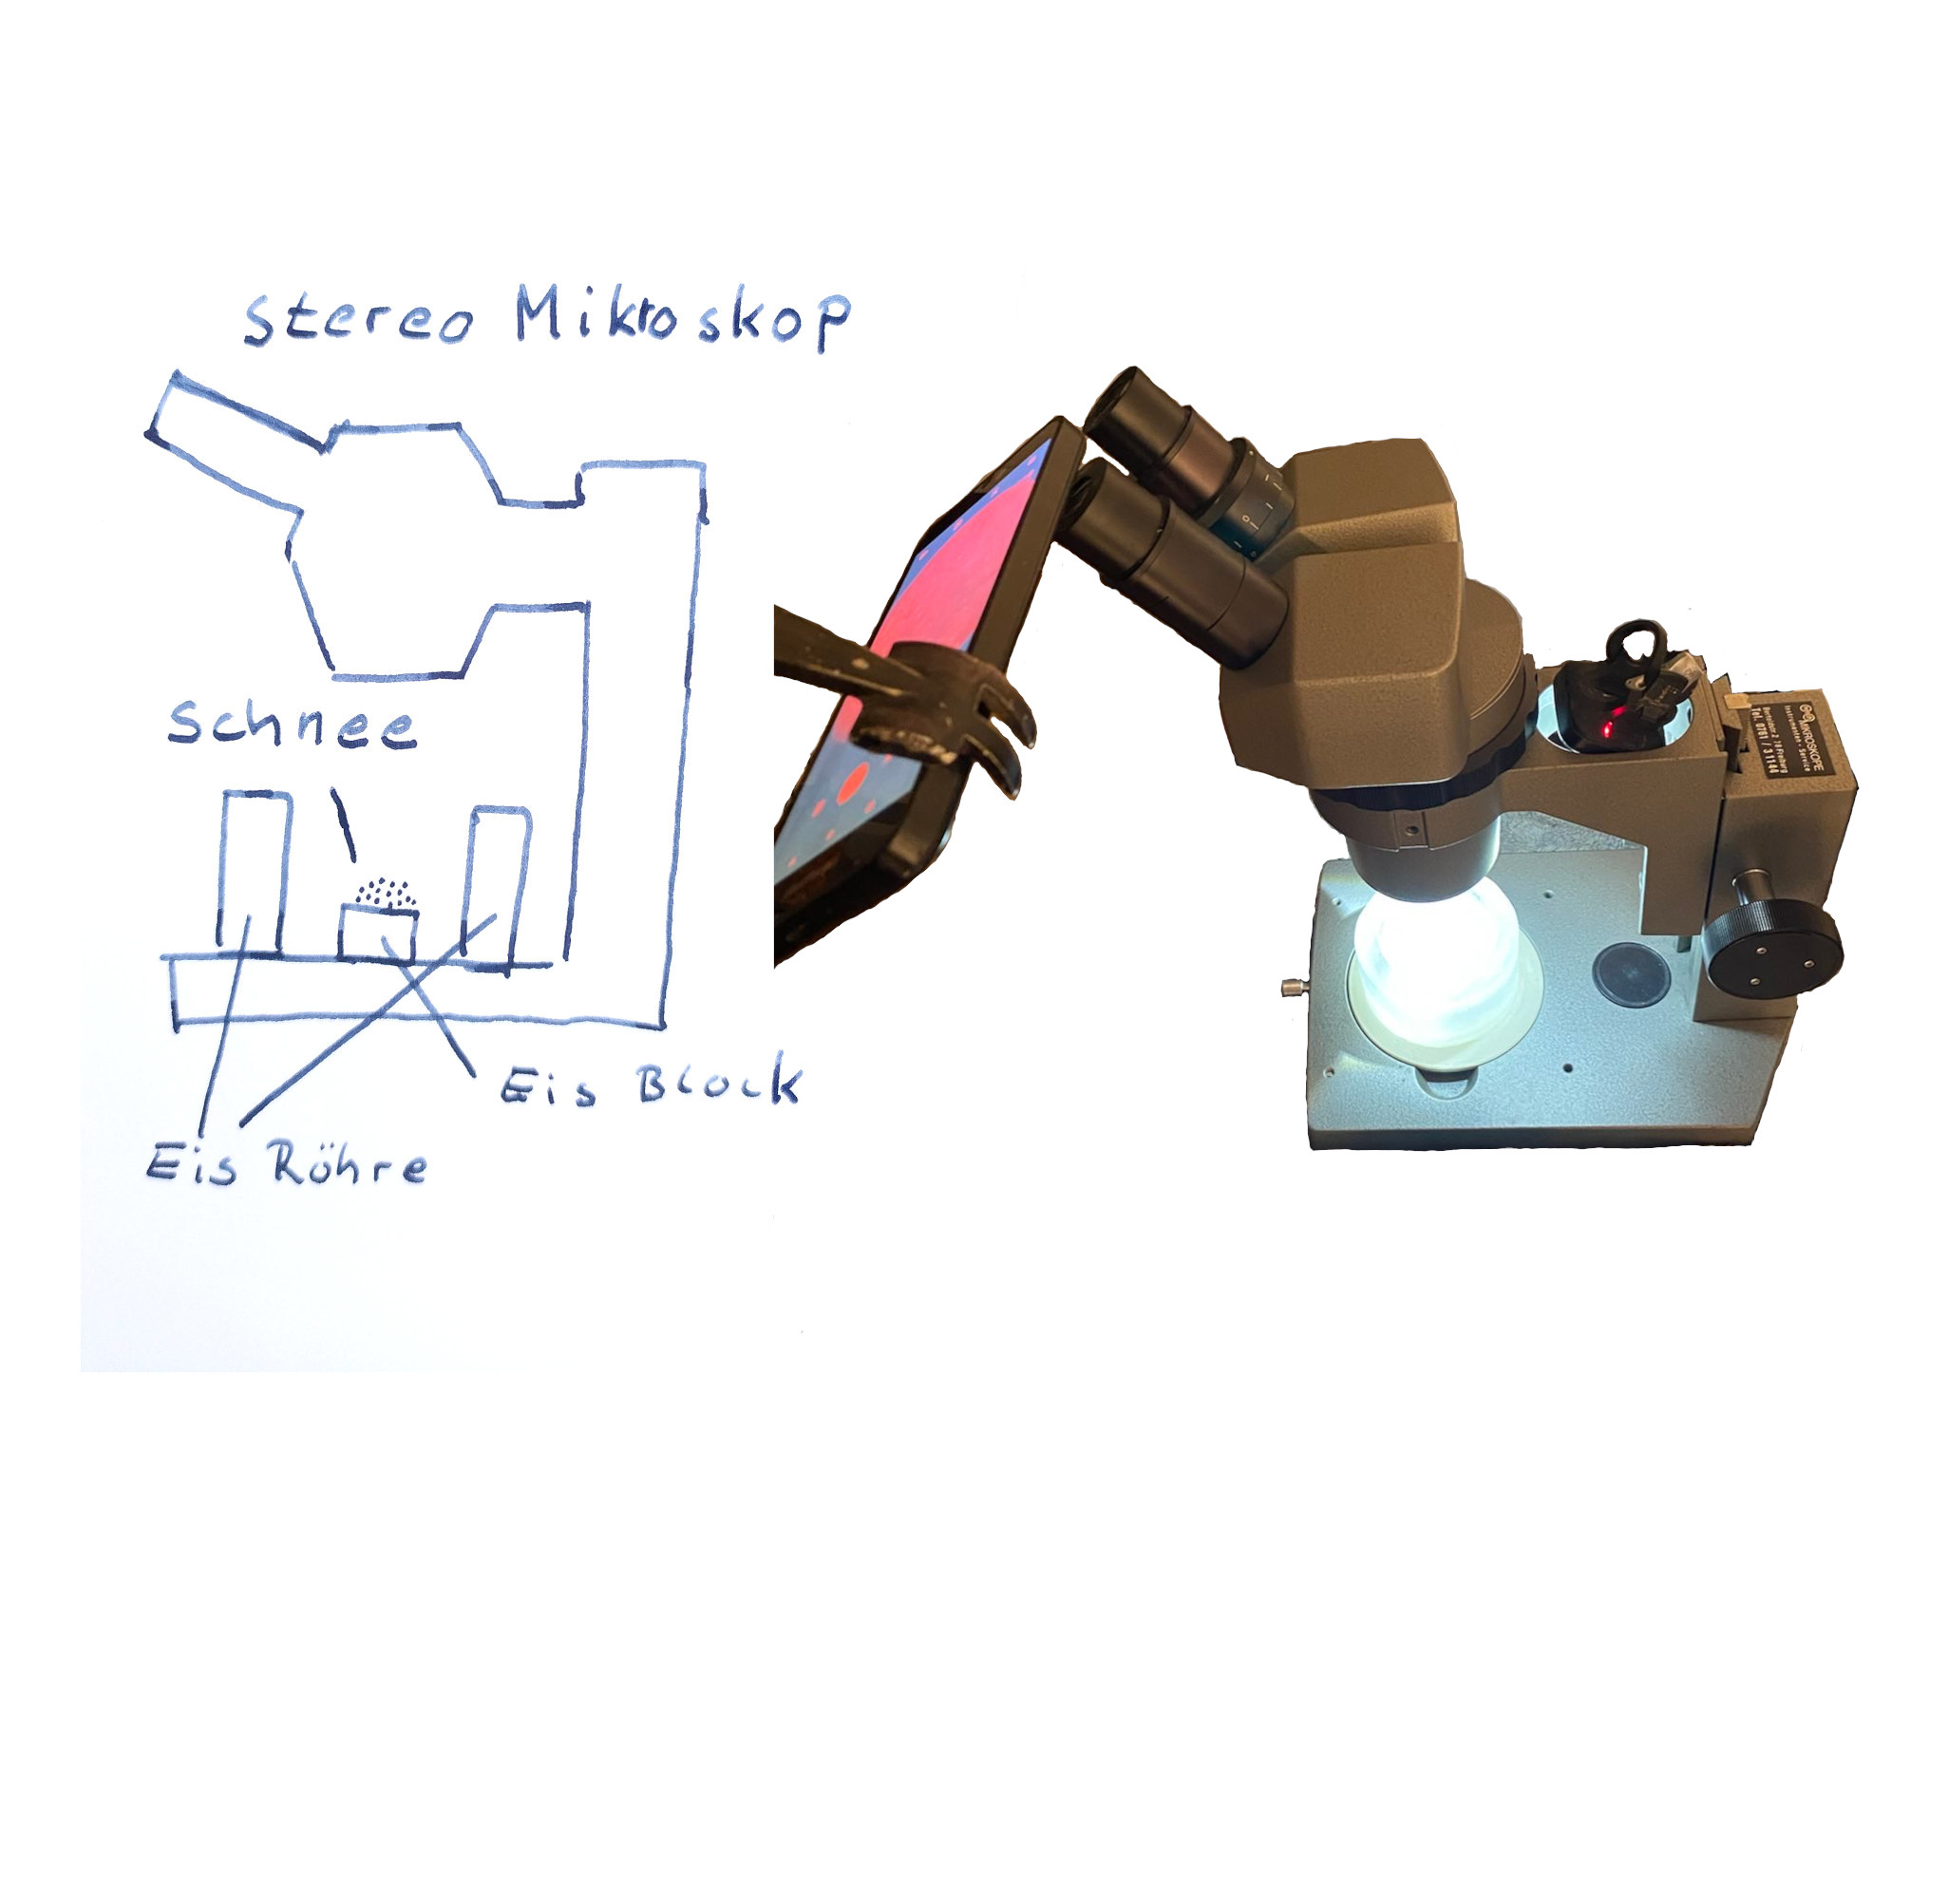
\includegraphics[width=0.8\textwidth]{Bilder/freistellen.jpeg}
    \caption{Aufbau einer Messung wo der Schnee durch eine Eisröhre gekühlt wird}
    \label{fig:AutMess}
\end{figure}
